%% The class cedram-ALCO is just a wrapper around amsart.cls (version 2)
%% implementing the layout of the journal, and some additionnal
%% administrative commands. 
%% You can place one option:
%% * "Unicode" if the file is UTF-8 encoded.
\documentclass[Unicode]{cedram-alco}


\usepackage{xcolor}


%% Here you might want to add some standard packages if those
%% functionnalities are required.
%\usepackage[matrix,arrow,tips,curve]{xy}
% ...
%% The production will anyway use amsmath (all ams utilities except
%% amscd for commutative diagrams which you need to load explicilty if
%% required), hyperref, graphicx, mathtools, enumitem...

%% User definitions if necessary...  Such definitions are forbidden
%% inside titles, abstracts or the bibliography.
\DeclarePairedDelimiter\abs{\lvert}{\rvert} %Something useful only for this sample's sake: you can erase this line in your file (or find it useful...)
%% The title of the paper: amsart's syntax. 
\title
%% The optionnal argument is the short version for headings.
[Exterior Algebra Tutte Functions]
%% The mandatory argument is for the title page, summaries, headings
%% if optionnal void.
{An Exterior Algebra Valued Tutte Function on Linear Matroid Pairs}

%% Authors according to amsart's syntax + distinction between Given
%% and Proper names:
\author[\initial{S.} \middlename{} Chaiken]{\firstname{Seth} \middlename{} \lastname{Chaiken}}

%% Do not include any other information inside \author's argument!
%% Other author data have special commands for them:
\address{University at Albany\\
  State University of New York\\
Computer Science Department\\
1400 Washington Avenue\\
Albany, NY 12222 (USA)}

%% Current address, if different from institutionnal address
\curraddr{18 Eileen Street\\
Albany, NY 12203 (USA)}


%% e-mail address
\email{schaiken@albany.edu}

%% possibly home page URL (not encouraged by journal's style)
%\urladdr{https://en.wikipedia.org/wiki/Marin\_Mersenne}

%% Acknowledgements are not a footnote in
%% \author, but are given apart:
%\thanks{The author was partially supported by a special grant for Junior Woodchucks.}


%% If co-authors exist, add them the same way, in alaphabetical order
%\author{\firstname{Joseph}  \lastname{Fourier}}
%\address{Universit\'e de  Grenoble\\
% Institut Moi-m\^eme\\
% BP74, 38402 SMH Cedex (France)}
%\email{fourier@fourier.edu.fr}

% Key words and phrases:
\keywords{Tutte Functions, Exterior Algebra, Laplacian, Electrical Networks}
  

%% Mathematical classification (2010)
%% This will not be printed but can be useful for database search
\subjclass{10X99, 14A12, 11L05}

%mycommands
\newcommand{\ext}[1]{\ensuremath{\mathbf{#1}}}
%\newcommand{\extvee}{\ensuremath{\mathbf{\vee}}}
\newcommand{\extvee}{\;\;}
\newcommand{\Plucker}{Pl\"{u}cker\ }

\newcommand{\Nal}{\ensuremath{N_{\alpha}}}
\newcommand{\NbePe}{\ensuremath{N_{\beta}^{\perp}}}
\newcommand{\eNal}{\ensuremath{\ext{N}_{\alpha}}}
\newcommand{\eNbePe}{\ensuremath{\ext{N}_{\beta}^{\perp}}}
\newcommand{\eNbe}{\ensuremath{\ext{N}_\beta}}
\newcommand{\Nbe}{\ensuremath{N_\beta}}

\newcommand{\Is}{\ensuremath{\iota}}
\newcommand{\Vs}{\ensuremath{\upsilon}}


%Emphasize in color!
\newcommand{\Remph}[1]{{\color{red}#1}}
\newcommand{\Bemph}[1]{{\color{blue}#1}}

\newcommand{\alert}[1]{{\color{red}#1}}



%\newcommand{\dunion}{\uplus}
\newcommand{\dunion}{\coprod}

\newcommand{\extLVert}[2]{\ext{L}\left( \begin{array}{c} {#1}\\ {#2} \end{array} \right)}
\newcommand{\extLVertSub}[3]{\ext{L}_{#1}\left( \begin{array}{c} {#2}\\ {#3} \end{array} \right)}
\newcommand{\extLHor}[2]{\ext{L}\left( {#1}\;\; {#2} \right)}
\newcommand{\extLHorSub}[3]{\ext{L}_{#1}\left(  {#2}\;\; {#3}  \right)}

\newcommand{\LVert}[2]{\ext{L}\left( \begin{array}{c} {#1}\\ {#2} \end{array} \right)}
\newcommand{\LVertSub}[3]{\ext{L}_{#1}\left( \begin{array}{c} {#2}\\ {#3} \end{array} \right)}
\newcommand{\LHor}[2]{\ext{L}\left( {#1}\;\; {#2} \right)}
\newcommand{\LHorSub}[3]{\ext{L}_{#1}\left(  {#2}\;\; {#3}  \right)}




\definecolor{Blue}{rgb}{.255,.41,.884} % RoyalBlue of svgnames
\definecolor{Red}{rgb}{1, 0, 0} % Red of svgnames
\definecolor{Green}{rgb}{.196,.804,.196} % LimeGreen of svgnames
\definecolor{Yellow}{rgb}{1,.648,0} % Orange of svgnames





\begin{document}
%% Abstracts must be placed before \maketitle
\begin{abstract}
 The matrix tree theorem expresses the basis enumeration Tutte function
(spanning tree count of connected graphic matroids) as a
determinant--a minor of the graph's Laplacian. We will generalize the
choice of a root vertex for the trees by distinguishing a fixed set $P$
of $p$ matroid elements, which we will call ports, a word from
engineering. We then define a function from $k$-linear matrix
representations of matroid pairs ($N_{\alpha},N_{\beta})$ (often
$N_{\alpha}=N_{\beta}$ whose ground sets
include $P$, into pure (decomposible)
exterior algebra elements which represent points in the Grassmannian of $p$ dimensional $k$-linear subspaces
of $k^{(2p)}$. We express this subspace value as a decomposible
(i.e. product of vectors) element in the exterior algebra (of
anti-symmetric tensors) over $k^{(2p)}$, in a standard way.  The result is
a restricted or set-pointed Tutte function $\ext{L}_E(N_{\alpha},N_{\beta})$
that
satisfies sign-corrected forms of the two familiar identities for
deletion/contraction of elements not in $P$, and for disjoint
union. Note that these identities are in exterior algebra, whose
multiplication is anti-commutative. This generalizes the all-minors
directed graph matrix tree theorem (proved combinatorially by the
author) because those minors are the coefficients in the expansion of
$T$'s value over the standard basis--they are the standardized Plucker
coordinates for the dimension $p$ subspace $T$'s value represents.  An
unusual feature for this Tutte-like function is that when $k$ is ordered
so the matroids are oriented, $T$ can distinguish different orientations
of the same matroid.  
\end{abstract}


\maketitle

% First paragraph after a section is not indented. If there is text
% below the title before the first section, it should be unindented
% like this.
\noindent
\input{gitcommit}

\section{Introduction}

\noindent
Tutte functions are a well-known, long-standing idea
for which new applications, variations and generalizations
continue to be active research subjects. For example,
Krajewski, Moffatt and Tanasa give a common Hopf algebra framework
for the deletion and contraction operations for many of
these variations\cite{KRAJEWSKI2018271}.
See also Crapo and Schmitt's work
on the Hopf algebra of matroids and call
for attention to ``naturally occurring algebraic
structures'' in matroid theory\cite{CRAPO20051066}.  The target for us
is exterior algebras, which occur naturally when problems of
Kirchhoff's and Ohm's law electrical network solving and their
generalizations are studied from a matroid theory point of view,
including a view from oriented matroids.  Besides its application
to differential forms, exterior algebra is
the algebra of the posing and solution of equations in elementary
linear algebra\cite{ExteriorAlgInLinalgRef}.


Our most compelling reason for connecting
Tutte functions with an exterior algebra (in lieu of a commutative
algebra) is that linear subspaces (as matroid representations and
solutions to systems of homogeneous linear equations)
are represented by exterior products of vectors; also called
\emph{decomposible} elements, \emph{decomposibles},
or ``pure'' antisymmetric tensors.
Our example of such subspaces
comprises solutions to problems posed from graphs that generalize inversion
of graph Laplacians.  To connect these with Tutte decomposition, we make
minor notational variations to the machinery of exterior algebra, also called Grassmann algebra,
as presented by Marcus\cite{MarcusFDMuAlPt2}.  First, we specify the particular basis $S$
so that a decomposible in the exterior algebra generated by $S$
can represent a matroid with ground set $S$.  Second, we specify a distinguished subset $P\subseteq S$
and our Tutte function will be valued in exterior algebras generated by sets related to $P$.
Third, as done with pseudo-forms\cite{Frankel}, we specify an orientation for each
space.

One of the earliest Tutte functions is the basis enumerator for matroids. It
is a determinant in the case of graphic, and more generally, regular matroids;
this is a consequence of the Cauchy-Binet theorem.
The well-known Matrix Tree theorem tells us this determinant is (up to sign)
any full-rank minor of the graph's Laplacian matrix. More generally,
every minor is an enumerator for forests (signed, in some non-principal minor
cases) satisfying the following condition: Each vertex indexing
a deleted row is in exactly one of the trees, and similary for each
vertex indexing a deleted column\cite{sdcMTT}.
(Each forest's sign depends on the sign of the
matching the forest determines between the deleted row vertices and
deleted column vertices; of course when the minor is principal,
the only such matching is the identity.  We will see that this variation of
sign is due to which oriented matroids are the result of contracting
the forest edges.)
We give a key observation: \emph{Each} such
minor, when $e$ is a given edge, equals the sum of the corresponding
minor when $e$ is deleted plus the determinant expansion terms for
forests that contain $e$.  The latter can be also be expressed as a determinant.
In the following, we will develop a formulation in which
\emph{all these minors together},
when they are constituted as an element in an exterior algebra, satisfy the
well-known Tutte identities.  The formulation applies to pairs of
row-spaces of matrices, with rank conditions for non-triviality,
and our Tutte decomposition operates on matrix
columns as does (possibly oriented)
matroid deletion and contraction.

In order for a tuple of determinants to be a Tutte function value, one
must label them in a combinatorial way.  For this purpose, we use
the \emph{set-pointed}\cite{TPMorphMatI99,TPMorphMatI99},
also called the
\emph{relative}\cite{RelTuttePolyDiaoHetyei} or
\emph{ported}\cite{sdcPorted,TutteEx}
variation of Tutte functions.
Let $P$ be a set.  A function $F$ is a $P$-ported
when the identity for deletion and contraction of $e$ is asserted,
and rules for reducing loops or coloops apply, only when $e \not\in P$.
$P$ will play the role of vertices in our all-minors of the Laplacian
matrix tree theorem specialization.
We prefer the engineering term ``port'' because it eludes to both an object through
which systems can be interconnected,
and can be manipulated and observed by their
environments\cite{Recski,narayanan1997submodular}.
Engineers would call our graph theory example (\ref{ExamK4}) a ``$p$-port'', with $p=2$.

Let $P_{\alpha}$ and $P_{\beta}$ be disjoint copies of $P$.  Let $K$ be a field.
We will see that our Tutte function's value will be an exterior product of
$|P|$ vectors in the $2|P|$ dimensional vector space over $K$ with basis $P_\alpha \cup P_\beta$.
I.e., our value will
have grade level or ``step''  $|P|$.
rank $2|P|$
As such, (when non-zero)
it is a \emph{Grassmann representitive}\cite{MarcusFDMuAlPt2}[p 18]
for some
dimension $P$ subspace, a point in the Grassmannian $Gr(|P|,2|P|)$.
However, in order for Tutte's additive identity to make sense, the value cannot be
a point in the $\binom{2|P|}{|P|}-1$ dimensional projective space
containing the variety $Gr(|P|,2|P|)$.  It must be in a module, which for
our construction is a linear space.

A possibly novel feature is that unlike the usual commutative ring values for Tutte
functions, our functions' values, being in an exterior algebra, are graded and have
\emph{anticommutative} multiplication.
Hence a sign correction must be included in Tutte's multiplicative
identity.  Our Tutte function merely reduces to the parametrized
basis enumerator obtained from setting, $u=v=0$ in Tutte
decomposition (\ref{ParamTutteEqGeneric})
with coloop $e$ valued at $g_e+r_eu$ and loop $e$ valued at $r_e+g_ev$.
``Porting'' is necessary for our approach to yield anything
interesting. To find a Tutte function, like the Whitney rank-nullity
generating function form in variables $u,v$, that reduces to our exterior
algebra version when $u=v=0$ is an interesting question.
Our
references\cite{MR0419272,SetPointedLV,sdcPorted,TutteEx,RelTuttePolyDiaoHetyei}
document that all the fundamental features
(expansions, universality, etc.)
of Tutte function theory extend to porting/set-pointing/relativization.  Throughout,
we restrict our attention to the ``normal'' parametrized Tutte functions which, according
to classifications given by Zaslavsky\cite{MR93a:05047},
and Bollobas and Riordan\cite{BollobasRiordanTuttePolyColored},
have rank-nullity generating function interpretations.
(They prove this requires the
coloop and loop values be what is above, with $u$, $v$ independent of $e$.)

Another possibly interesting feature is that, in a rather trivial way,
our Tutte function can distinguish different orientations of an oriented
matroid.  When decomposition defined by our Tutte identities is applied to
a represented oriented matroid, the irreducibles are representations of
some of its minors for which their ground set only contains elements in $P$.
Hence different orientations of the same matroid minor are distinguished.  Recently,
a new Tutte function variation that distinguishes properties of orientations
more finely was found\cite{AwanBernardiOMTuttePre}.

Parameters $r_e$, $g_e$ are given for each element $e\not\in P$. We
will have, formally,
\begin{equation}\label{ParamTutteEqGeneric}
   F(N) = g_eF(N/e)+r_eF(N\backslash e) \text{ if\ }e\text{ can be deleted and contracted, and }e\not\in P.
\end{equation}
Indeed, our chief motivation is to give an algebraic combinatorial description of solutions
to electrical network problems, where the parameters will represent the coefficient
in Ohm's law.  It is convenient (and elegant) to write that law in homogeneous form:
For each resistor $e$ there
are two parameters $r_e,g_e$
(``proresistance'', ``proconductance'' apparently originated in \cite{SmithElec} and  used in
\cite{TutteEx,CirThProjHomo2019}) such that the current and voltage drop
combination of a resistor $(i_e,v_e)$ $=$ $x(g_e,r_e)$ for some $x$.
In other words, when they
are non-zero and not infinite, the conventional
resistance is $r_e/g_e$ and conductance is $g_e/r_e$\footnote{Electrical engineers
sometimes call these reciprocal quantities ``impedance'' and ``admittance'' especially
when they are in $\mathbb{C}$.}. Shorts (zero resistance) and opens (zero
conductance) are thus accomodated.   To make this long story short (see section ()),
our Tutte function's value
will encode the set of voltage drops across and current flows through each of
the network edges in $P$ that are compatible with Kirchhoff's and Ohm's laws applied to $E\cup P$. This set
is the linear solution space of an underdetermined system projected into the
dimension $2|P|$ space with a voltage ($v_{p}$) and a current ($i_{p}$) coordinate for each $p\in P$.

Thus, the subspace represented by our Tutte function's value is parametrized.  This opens
questions for research into the topological and geometric properties of the set of those subspaces
as the parameters range say over $\mathbb{R}$ or $\mathbb{C}$, say for a given graph or pair of
matrices.



\section{Setup and Theorem}

\noindent
In applications, columns of our full-row-rank matrices will be labelled by elements representing
or related to matroid ground set elements, and to generators of our exterior algebras.
Thus the row space is encoded by the exterior product of the row vectors. Matroid, and,
in the case of graphic matroids, graph operations will involve these elements.   

For clarity and simplicity, we demonstrate this with matrices and
and give the example of solving the electrical network equations for a graph.

The Tutte function is defined
on pairs of decomposibles.
The explicit vectors
or matrices do not play a role except in applications.

It is important to recognize that the two given decomposibles, and the Tutte function's
value, are decomposible exterior algebra elements,
not the point in the Grassmannian
whose \Plucker coordinates are equivalence classes of non-zero multiples.
We \emph{do} distinguish different such multiples.  Another way
to put it is that our data and constructed objects are matrices modulo left multiplication
by $SL_r$, not by $GL_r$ the latter which gives the Grassmannian.
Of course all such matrix classes surject onto the Grassmannian.


Let $\Nal$ and $\NbePe$ be two full row rank matrices (over field $K$)
with columns indexed by $P\cup E$, $P\cap E=\emptyset$,
for which $\text{rank}(\Nal)+\text{rank}(\NbePe)=|E|+|P|$.
Let
$G=\text{diag}\{g_e\}_{e\in E} $ and $R=\text{diag}\{r_e\}_{e\in E}$
be diagonal matrices of parameters.  For any such matrix $N$, $N(E)$ and
$N(P)$ denote the submatrices with columns $E$ and $P$ respectively. With
two disjoint copies of $P$ and bijections
$P \leftrightarrow P_{\alpha}\leftrightarrow P_{\beta}$, define the matrix
with columns indexed by $P_\alpha \dunion P_\beta \dunion E$, where each entry
is in $K$ or is a $K$ multiple of a parameter:
\begin{equation}\label{LmatrixDef}
    L = L\left(\begin{array}{cc} {\Nal} \\ {\NbePe}  \end{array}\right)
    = \left[\begin{array}{c|c|c} \Nal(P)  &  0  &  \Nal(E)G \\  \hline
        0  & \NbePe(P)  &  \NbePe(E)R \end{array}\right].
\end{equation}

The remaining two steps below will simply take the exterior product of the rows of $L$, and
then, for the value,
extract the terms that are divisible by $\wedge_{e \in E}\ext{e}$
when the product
is expanded in terms of the exterior algebra basis
generated by $P_\alpha \dunion P_\beta \dunion E$.
(Some will recognize the latter step, up to sign, as interior product, when elements
of $E$ are dual to the column index elements.  We choose notation
so that the sign complies with oriented matroid practice\cite{OMBOOK} and
because the generators of the codomain exterior algebra no longer include $E$.
We'll use the same operation for contraction, below.)
This is too simple because it remains unclear how to define the construction for the
``minors'' (to be defined) which will have smaller sets in place of $E$. The
construction must be consistent on the minors in order that the values
of our function on those minors satisfy the Tutte identities. 

It is easy to explain this construction when it is weakened
so it applies to Grassmannians:
Project the solution space $\{z\}$ of $Lz=0$ onto
the $P_\alpha\dunion P_\beta$ coordinates and then take the projection's orthogonal
complement with respect to this coodinate  basis.
In other words, we eliminate all the variables
indexed by $E$ in the system $Lz=0$ and take the exterior product of the rows
from the result of the elimination; the result is a 
representitive (ambiguously defined) for point in the Grassmannian.
Such a result is nice for solving for some of the remaining $z$'s in terms of
the others, but a failure
for the additive or multiplicative Tutte identities.


\subsection{Definition of a Tutte Function of $P$-Ported Pairs}


We need 
some careful formalism so we can algebraically relate the resulting Tutte function value
to its values for our to-be-defined minors and direct product factors.  Those 
will have a proper subset for $E$ and possibly so for $P$.

Let $U$ be the vector space $K(g_e,\ldots;r_e,\ldots)P_\alpha
\dunion P_\beta \dunion E$ with distingushed basis $P_\alpha
\dunion P_\beta \dunion E$.  Vectors and other elements of the
exterior algebra $\wedge U$ will be denoted by boldface
characters, such as $\ext{e}_j$, $\ext{p_\alpha}_k$,
$\ext{p_\beta}_l$ $\in$ $P_\alpha \dunion P_\beta \dunion E$.
    
Let $p = |P|$, $n=|E|$ and $L_i$ be row $i$ of $L$ for $i\in\{1,\ldots,n+p\}$.
We form $\ext{L}$ by exterior multiplication (in order) of the vectors each given by the
rows of $(n+p)\times (n+2p)$ matrix $L$ for the coefficients when written in terms of
basis $P_\alpha \dunion P_\beta \dunion E$:
\begin{equation}\label{defExtL}
  \ext{L} = \wedge_{i=1}^{n+p}L_i
      [\ext{p_\alpha}_1\ \cdots\ \ext{p_\alpha}_{p}\ \ext{p_\beta}_1\ \cdots\ \ext{p_\beta}_{p}\
      \ext{e}_1\ \cdots\ \ext{e}_{n}]^t. 
\end{equation}

We can now define what will turn out to be our Tutte function.  One cannot say what it means for
it to be a Tutte function until we get to defining the deletion and contraction operations!

Let us fully expand $\ext{L}$ into a polynomial in anti-commuting variables
$P_\alpha \dunion P_\beta \dunion E$.  Since $\ext{v}\wedge\ext{w}=-\ext{w}\wedge\ext{v}$ for vectors in
exterior algebra, we can write
\[
\ext{L} = (\ext{L}_E)\wedge (\ext{e_1}\wedge\ext{e_2}\cdots\wedge\ext{e_n}) + \ext{J}.
\]
We will abbreviate expressions like $(\ext{e_1}\wedge\ext{e_2}\cdots\wedge\ext{e_n})$ by
$(\ext{e_1}\ext{e_2}\cdots\ext{e_n})$ or $\ext{E}$ where \emph{set $E$ is specified as a sequence of its elements}.
So, given $(N_\alpha,N_\beta^\perp)$ as above, $\ext{L}_E(N_\alpha,N_\beta^\perp)$ is defined by (\ref{defExtL}) where
$\ext{J}$ is the sum of terms none of which is a multiple of $\ext{E}$.
In other words, $\ext{L}_E$ is the image of the homomorphism
$\Gamma_E:\wedge^{(2p+n)}U\rightarrow\wedge^{(2p)}U$ defined on the basis of
products of vectors corresponding to $P_\alpha \dunion P_\beta \dunion E$ to that
of $P_\alpha \dunion P_\beta$ as follows:
\[
   \begin{array}{ccc}
     \ext{Z}\ext{E} & \longmapsto & \ext{Z} \\
     \ext{Z}\ext{E'} & \longmapsto & 0
   \end{array}
\]
where $Z\subseteq P_\alpha \dunion P_\beta$ and $E'\subsetneqq E$.

\begin{prop}
  $\ext{L}_E(N_\alpha,N_\beta^\perp)$ is invariant under left actions of $SL_r$ on $N_\alpha$ or $N_\beta^\perp$.
\end{prop}
\begin{proof}
  All the coefficients are products of an all row minor of $N_\alpha$, an all-row minor of $N_\beta^\perp$, a sign, and
  parameters.
  By definition, the actions of $SL_r$ will multiply those determinants by 1. 
\end{proof}

We can therefore use the similarly formed exterior products
(respecting order) of the rows of $N_\alpha$ and $N_\beta^\perp$
for our data, denote them by 
$\ext{N_\alpha}$ and $\ext{N_\beta^\perp}$
and justify

\begin{defi}
  Given $E$, $P$ and $(\ext{N_\alpha},\ext{N_\beta^\perp})$ as above,
  $\extLVertSub{E}{\ext{N_\alpha}}{\ext{N_\beta^\perp}}$ is the
  unique exterior algebra element satisfying
  \[
  \extLVert{\ext{N_\alpha}}{\ext{N_\beta^\perp}}=
  (\ext{L}_E)\wedge (\ext{e_1}\wedge\ext{e_2}\cdots\wedge\ext{e_n}) + \ext{J} =
  (\extLVertSub{E}{\ext{N_\alpha}}{\ext{N_\beta^\perp}})\ext{E}+\ext{J},
  \]
where $\ext{J}$ is the sum of terms none of which is a multiple of
$\ext{E}=\ext{e_1}\wedge\ext{e_2}\cdots\wedge\ext{e_n}$, when
$\ext{L}$ is expanded using the basis generated by $P_\alpha \dunion
P_\beta \dunion E$.  In other words,
  \[ 
  \extLVertSub{E}
              {\ext{N_\alpha}}
              {\ext{N_\beta^\perp}}
              =
              \Gamma_E(
              \extLVert{\ext{N_\alpha}}{\ext{N_\beta^\perp}}).
  \]
\end{defi}


\subsection{Example and an interpretation of $\ext{L}_E(\ext{N_\alpha},\ext{N_\beta^\perp})$}\label{ExamK4}

With the complete graph $G=K_4$, we will illustrate our construction,
its evaluation and an interpretation
in terms $G$'s familiar linear spaces, oriented matroids, and electrical
network problem model.  $P=\{p_1, p_2\}$ is comprised of two non-adjacent
edges and the rest, $K_{2,2}$, will comprise $E$.  

We relate $K_4$ as a 1-dimensional abstract simplicial complex to
its role as an electrical network model.
To make cycles represent flows of positive current,
coboundaries electrical potentials and resistance positive,
our sign conventions for arbitrarilly oriented labeled (multi)graphs
will be \emph{opposite that of} the homology of 1-dimensional chain complexes:
For $e : a \rightarrow b$, $\partial_1(e)=a-b$, $\partial^0(\hat{a})=\hat{e}+ \ldots\  $,
$\partial^0(\hat{b})=-\hat{e}+ \ldots\  $, where $e$ is edge with end vertices $a$ and $b$ oriented
as indicated\
\footnote{
On the other hand, for the sake of mathematical simplicity,
we will use this sign convention the port edges (in $P$).
In electrical engineering
circuit theory writings the sign convention for ports is reversed
so quantities characterizing typical system behavior
observable at the ports
are positive.}.
With $\partial^0(\phi(\hat{a}) \hat{a} + \phi(\hat{b}) \hat{b}) = (\phi(\hat{a})-\phi(\hat{b}))\hat{e} + \cdots$,
$\phi(\hat{a})-\phi(\hat{b})$ is the voltage drop going from $a$ to $b$.
Edge sets $E$ and $P$ will respectively represent resistors and ports.
When $e\in E$,
Ohm's law says that
$\phi(\hat{a})-\phi(\hat{b})$ times the resistance of $e$ equals the current through $e$,
flowing from $a$ to $b$.
For us, the currents through and voltage drops along
in all these edges are variables $i_t$ and $v_t$ for $t\in P\cup E$.  Ohm's law
is asserted in the homogeneous form:  For $e\in E$, the voltage-drop-to-current ratio
$v_e:i_e$ $=$ $r_e:g_e$, the ratio of the resistivity parameters.
Those parameters are not given for ports.
Kirchhoff's voltage law asserts that $\sum_tv_t\hat{t}$ is the 1-coboundry $\partial^0(\sum \phi(\hat{a})\hat{a})$
for some $\phi:V\rightarrow K$; physically, $\phi$ is the electrical potential function.
Kirchhoff's current law asserts that $\sum_ti_t t$ is a 1-cycle, i.e., in $\text{ker }\partial_1$. 
The problem of linear electrical network analysis is to characterize
the linear relationships among port current and voltage drop variables implied by
the network topology, Kirchhoffs' and Ohm's laws.  


Let $P=\{p_1, p_2\}$ and $E=\{e_1, e_2, e_3, e_4\}$ together be the edges in the (oriented) graph
below representing an electrical network, where $E$ represents the resistors.   $N_\alpha$ is
a full-row-rank, all-column submatrix of the matrix form for $\partial^1$.  It is the
usual ``signed'' vertex-edge incidence matrix which represents our graph's graphic matroid, with one
row deleted so $N_\alpha$ has full row rank.  The rows of $N_\alpha$ hold the coefficients in
Kirchhoff's current law, asserting that the edge currents constitute a 1-cycle, (i.e., a flow.)
$N_\beta^\perp$ is a totally unimodular matrix whose
rows are a basis for the 1-cycle space, conveniently
obtainable by coding the incidences of edges with the oriented fundamental
circuits each associated to an edge not in a fixed spanning tree.
Its rows hold the coefficients in
Kirchhoff's voltage law, asserting that the edge
voltages drops constitute a 1-coboundary, differences
of a potential along edges.
This well-known construction gives
two full row rank totally unimodular matrices whose row spaces are orthogonal complements,
representing our graph $G$'s
graphic (with bases $\mathcal{B}(G)$) and cographic matroids respectively.

\begin{figure}
  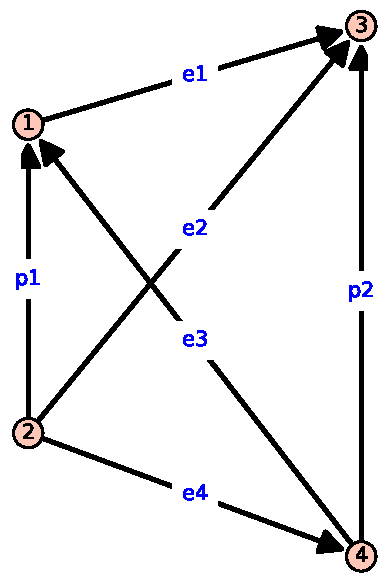
\includegraphics[scale=0.5]{K4.pdf}
\end{figure}

We begin with the familiar incidence matrix representation of K4's matroid.
We delete row 2 and take a representation for the dual that is consistent
with our exterior algebra duality operator (\ref{}):


\[
\left(\begin{array}{cc|cccc}
1 & 0 & -1 & 0 & 1 & 0 \\
-1 & 0 & 0 & -1 & 0 & -1 \\
0 & 1 & 1 & 1 & 0 & 0 \\
0 & -1 & 0 & 0 & -1 & 1
\end{array}\right)
\;\;\;
N_\alpha=
\left(\begin{array}
{cc|cccc}
1 & 0 & -1 & 0 & 1 & 0 \\
0 & 1 & 1 & 1 & 0 & 0 \\
0 & -1 & 0 & 0 & -1 & 1
\end{array}\right)
%\]
\;\;\;\;
%\[
N_\beta^\perp =
\left(\begin{array}{cc|cccc}
1 & 0 & 0 & 0 & -1 & -1 \\
0 & 1 & 0 & -1 & 0 & 1 \\
0 & 0 & 1 & -1 & 1 & 1
\end{array}\right)
\]


We form the following system of equations according to (\ref{LmatrixDef}).

\begin{equation}\label{K4Equation}
\begin{split}
  0=L\left(\begin{array}{cc} {\Nal} \\ {\NbePe}  \end{array}\right)z
    =& \left[\begin{array}{c|c|c} \Nal(P)  &  0  &  \Nal(E)G \\  \hline
        0  & \NbePe(P)  &  \NbePe(E)R \end{array}\right]
    \left[ \begin{array}{c} i_{p_1} \\ i_{p_2} \\ v_{p_1} \\ v_{p_2} \\ x_{e_1} \\ x_{e_2} \\ x_{e_3} \\ x_{e_4}
      \end{array}
      \right]
    \\
    =&
\left(\begin{array}{cc|cc|cccc}
1 & 0 & 0 & 0 & -g_{1} & 0 & g_{3} & 0 \\
0 & 1 & 0 & 0 & g_{1} & g_{2} & 0 & 0 \\
0 & -1 & 0 & 0 & 0 & 0 & -g_{3} & g_{4} \\ \hline
0 & 0 & 1 & 0 & 0 & 0 & -r_{3} & -r_{4} \\
0 & 0 & 0 & 1 & 0 & -r_{2} & 0 & r_{4} \\
0 & 0 & 0 & 0 & r_{1} & -r_{2} & r_{3} & r_{4}
\end{array}\right)z
\end{split}
\end{equation}


The electrical network problem at hand is to determine linear constraints on the
port variables $i_p, v_p$, $p\in P = \{p_1, p_2\}$ imposed by the system.  In other words,
we want a linear map $M$ on the $K$-vector space with basis $P_\alpha, P_\beta$ whose kernel
is the projection of this system's solution space.
Below is a solution.
We set $r_e=1$ for $e\in E$, and $D=g_{1} g_{2} g_{3} + g_{1} g_{2} g_{4} + g_{1} g_{3} g_{4} + g_{2} g_{3} g_{4}$.
\begin{equation}\label{K4Soln}
M\left(\begin{array}{c} i_{p1} \\ i_{p2} \\ v_{p1} \\ v_{p2}
\end{array}\right) =
\left(\begin{array}{cccc}
{\left(g_{1} + g_{2}\right)} {\left(g_{3} + g_{4}\right)} & -g_{2} g_{3} + g_{1} g_{4} & D & 0 \\
-g_{2} g_{3} + g_{1} g_{4} & {\left(g_{1} + g_{3}\right)} {\left(g_{2} + g_{4}\right)} & 0 & D
\end{array}\right)
\left(\begin{array}{c} i_{p1} \\ i_{p2} \\ v_{p1} \\ v_{p2}
\end{array}\right) = 0
\end{equation}


To compute $\ext{L}_E$ from its definition, set 
$z=[\ext{p}_{\alpha 1},\ext{p}_{\alpha 2},\ext{p}_{\beta 1},\ext{p}_{\beta 2},
  \ext{e}_1,  \ext{e}_2,  \ext{e}_3,  \ext{e}_4]^t$
in the right hand side of (\ref{K4Equation}) 
and expand in terms of this basis
the exterior product (in order) of the resulting column's entries.
Finally, we select
the terms that can be expressed as $\ext{T}\ext{e}_1\ext{e}_2\ext{e}_3\ext{e}_4$.  The final
value is the sum of such $\ext{T}$.
Each $\ext{T}$ is the $\wedge$ of unique pair of distinct elements
of $\{\ext{p}_{\alpha 1}, \ext{p}_{\alpha 2}, \ext{p}_{\beta 1}, \ext{p}_{\beta 2}\}$
with a coefficient that is a polynomial in the 
$g_e$, $r_e$.  These coefficients are \Plucker coordinates
for the orthogonal complement of the electrical network
(itself parametrized by the $g_e, r_e$) solution space.
Each polynomial
term encodes a subset of $E=\{e_1, e_2, e_3, e_4\}$, for example, $\{e_1, e_2\}$ is encoded
by $g_1g_2r_3r_4$. Note that each coefficient enumerates
the common bases of a pair of not always distinct of matroid minors.


\begin{equation}\label{K4table}
\begin{array}{|c|c|c|} \hline
\text{basis element} & \text{coefficient} & \text{enumerates bases}\\
  \hline

\ext{p}_{\alpha 1}\ext{p}_{\alpha 2} &
g_1 + g_2 + g_3 + g_4 & \mathcal{B}(G/\{p_1, p_2\})

\\ \hline

\ext{p}_{\alpha 1}\ext{p}_{\beta 1} &
g_2g_3 - g_1g_4 &  \mathcal{B}(G/p_1\setminus p_2)\cap\mathcal{B}(G/p_2\setminus p_1)

\\ \hline

\ext{p}_{\alpha 1}\ext{p}_{\beta 2} &
(g_1 + g_2)(g_3 + g_4) & \mathcal{B}(G/p_1\setminus p_2)
\\ \hline 

\ext{p}_{\alpha 2}\ext{p}_{\beta 1} & -(g_1 + g_3)(g_2+g_4) & \mathcal{B}(G/p_2\setminus p_1)
\\ \hline
 
\ext{p}_{\alpha 2}\ext{p}_{\beta 2} &
-g_2g_3 + g_1g_4 & \mathcal{B}(G/p_1\setminus p_2)\cap\mathcal{B}(G/p_2\setminus p_1)
\\ \hline
 
\ext{p}_{\beta 1}\ext{p}_{\beta 2} &
g_1g_2g_3 + g_1g_2g_4 + g_1g_3g_4 + g_2g_3g_4 & \mathcal{B}(G\setminus \{p_1, p_2\})
\\ \hline

\end{array}
\end{equation}

To verify that the coefficients of our $\ext{L}_E$
in (\ref{K4table}) are \Plucker coordinates, and
indeed that $\ext{L}_E$ represents the space of
linear constraints for the
network solution problem,
one can calculate that each $2\times 2$ minor of the matrix in
(\ref{K4Soln}) equals the $D$ multiple of the corresponding coefficient
in  (\ref{K4table}).  The one non-trivial calculation is
\[
{\left(g_{1} + g_{2}\right)} {\left(g_{1} + g_{3}\right)} {\left(g_{2} + g_{4}\right)} {\left(g_{3} + g_{4}\right)} - {\left(-g_{2} g_{3} + g_{1} g_{4}\right)}^{2} = D(g_1+g_2+g_3+g_4)
\]

This example also demonstrates that $\ext{L}_E$ might not have a
matrix representation all of whose entries are $K_0$ polynomials in the $r_e, g_e$.

\subsection{Example with $\ext{N}_\alpha\neq\ext{N}_\beta$}
We take $N_\alpha$ from before, but form $N_\beta$ from $N_\alpha$ by replacing $-1$s by $0$.
$N_\beta$ now represents the partition matroid $\Pi$ where
each edge in a basis has its head incident to one distinct vertex in $\{1, 3, 4 \}$.


\[
N_\alpha=
\left(\begin{array}
{cc|cccc}
1 & 0 & -1 & 0 & 1 & 0 \\
0 & 1 & 1 & 1 & 0 & 0 \\
0 & -1 & 0 & 0 & -1 & 1
\end{array}\right)
%\]
\;\;\;\;
%\[
N_\beta=
\left(\begin{array}
{cc|cccc}
1 & 0 & 0 & 0 & 1 & 0 \\
0 & 1 & 1 & 1 & 0 & 0 \\
0 & 0 & 0 & 0 & 0 & 1
\end{array}\right)
\;\;\;
N_\beta^\perp =
\left(\begin{array}{cc|cccc}
1 & 0 & 0 & 0 & -1 & 0 \\
0 & 1 & 0 & -1 & 0 & 0 \\
0 & 0 & 1 & -1 & 0 & 0
\end{array}\right)
\]


\begin{equation}\label{K4Dirtable}
\begin{array}{|c|c|c|} \hline
\text{basis element} & \text{coefficient} & \text{enumerates bases}\\
  \hline

\ext{p}_{\alpha 1}\ext{p}_{\alpha 2} &
 g_{4} & \mathcal{B}(G/\{p_1, p_2\}) \cap  \mathcal{B}(\Pi/\{p_1, p_2\})

\\ \hline

\ext{p}_{\alpha 1}\ext{p}_{\beta 1} &
0 &  \mathcal{B}(G/p_1\setminus p_2)\cap\mathcal{B}(\Pi/p_2\setminus p_1)

\\ \hline

\ext{p}_{\alpha 1}\ext{p}_{\beta 2} &
 (g_{1} +  g_{2}) g_{4} & \mathcal{B}(G/p_1\setminus p_2)  \cap \mathcal{B}(\Pi/p_1\setminus p_2)
\\ \hline 

\ext{p}_{\alpha 2}\ext{p}_{\beta 1} &
- g_{3} g_{4} & \mathcal{B}(G/p_2\setminus p_1) \cap \mathcal{B}(\Pi/p_2\setminus p_1)
\\ \hline
 
\ext{p}_{\alpha 2}\ext{p}_{\beta 2} &
 g_{1} g_{4} & \mathcal{B}(G/p_1\setminus p_2)\cap\mathcal{B}(\Pi/p_2\setminus p_1)
\\ \hline
 
\ext{p}_{\beta 1}\ext{p}_{\beta 2} &
 (g_{1} +g_{2}) g_{3} g_{4} & \mathcal{B}(G\setminus \{p_1, p_2\})  \cap \mathcal{B}(\Pi\setminus \{p_1, p_2\})
\\ \hline

\end{array}
\end{equation}





\subsection{An easy but weak Tutte function variation}

This is apparent:  Take any $e\in E$, any parameter
values and $E'=E\setminus e$. Generalizing the example's discussion tells us that all three of
(1) $\ext{L}_E(\ext{N_\alpha},\ext{N_\beta^\perp})$,
(2) $\ext{L}_{E'}(\ext{N_\alpha}/e,\ext{N_\beta^\perp\setminus e})$ and
(3) $\ext{L}_{E'}(\ext{N_\alpha}\setminus e,\ext{N_\beta^\perp/e})$ represent
\Plucker coordinates, because they are representatives for the \Plucker coordinates
of the row spaces of the $F$'s from (1), (2) and (3) respectively.  Since \emph{for each determinant
$D_1$, $D_2$ and $D_3$ separately} in their expansions $c_1 D_1 = c_2 g_e D_2 + c_3 r_e D_3$ for
some coefficients, we can say:

\begin{prop}
Let $G_1$, $G_2$ and $G_3$ be points on the Grassmannian $Gr(p,2p)$ represented by
$\ext{L}_E(\ext{N_\alpha},\ext{N_\beta^\perp})$,
$\ext{L}_{E'}(\ext{N_\alpha}/e,\ext{N_\beta^\perp\setminus e})$ and
$\ext{L}_{E'}(\ext{N_\alpha}\setminus e,\ext{N_\beta^\perp/e})$ respectively. Then
$G_1$, $G_2$ and $G_3$ are colinear in the projective space containing this Grassmannian, and
all points on the line determined by $G_2$, $G_3$ represent points in this Grassmannian.
\end{prop}
\begin{proof}
  As $(r_e:g_e)$ ranges over $\mathbb{P}^1(k)$, $\ext{L}_E(\ext{N_\alpha},\ext{N_\beta^\perp})$, the
  exterior algebra element representing the row space of a matrix, remains a Grassmann representitive.
\end{proof}

\newpage

\section{Algebraic Formulation and Proof}

We naturally take Hodge star for the operation on
decomposibles that represents dualization of their
matroids.
However, the minors and
(nontrivial) direct product factors of matroid $M$
have ground sets that are proper subsets of $M$'s ground set.
We just postulate an orientation for \emph{every} finite set.
For simplicity, the same symbol $\epsilon$ is used throughout.
Exterior algebra operations
representing matroid deletion and contraction will therefore
be consistent with the operation for duality by using our
global orderings $\epsilon$ for our Hodge star.

We do not put conditions to relate our orientations of
of different sets.  Our formulas that involve two ordered sets $S_1$
and $S_2$ will therefore include the factor $\epsilon(S_1)\epsilon(S_2)$.




In the following formulas, $A$, $B$ and $\overline{B}$ are
sets expressed as sequences.
\begin{defi}\label{extmatdefs}
    \[
    \begin{array}{cc}
\text{deletion\ } \bullet\backslash A  & \text{restriction}  \\
\text{contraction\ }\bullet / A             & \ext{N}/A:B\mapsto\ext{N}[BA]\\
\text{duality\ }\bullet^{\perp} &
\ext{N}^{\perp}:B\mapsto\ext{N}[\overline{B}]\epsilon(\overline{B}B)
    \end{array}
    \]
\end{defi}
    In the definition of duality, $B$ is ordered,
    but $\overline{B}$ is an arbitrary ordering of the complement of $B$
    with respect to the ground set of $\ext{N}$.
    The result is unchanged for all reorderings of $\overline{B}$,
    so dualization is well-defined.  It represents linear matroid duality
    since Hodge star maps a subspace $V$'s representitive to a representitive
    of the orthogonal complement of $V$ when the basis defining it is
    declared to be orthonormal, see, e.g.\cite{MarcusFDMuAlPt2}.



\begin{prop}
  Let $S$ be the ground set for $\ext{N}$.
  Let $X$ be a sequenced subset of $S$.
  Let $S'$ be any sequencing of $S\backslash X$.
    \begin{equation} (\ext{N}\backslash X)^\perp = \epsilon(S')\epsilon(S'X)(\ext{N}^\perp/X)
    \end{equation}
    \begin{equation} (\ext{N}/X)^\perp = \epsilon(S')\epsilon(S'X)(-1)^{|X|r\ext{N}^\perp}(\ext{N}^\perp\backslash X)
    \end{equation}
\end{prop}
\begin{proof}
  Apply the definitions.  These dualization formulas are well-defined since they
  are unchanged over different sequencings of $S'$.
\end{proof}

To facilitate proofs, we introduce equivalent definitions to avoid explicit matrices.
\begin{defi}
  $\Is_G$ and $\Vs_R$ are exterior algebra homomorphisms depending on our commuting parameters
  $\{g_e, r_e\}$ generated by
  the following actions on $\ext{e}_i\in E$ and $\ext{p}_j\in P$:
  $\Is_G(\ext{e}_i)= g_{e_i}\ext{e}_i$, $\Vs_R(\ext{e}_i)=r_{e_i}\ext{e}_i$,
  $\Is_G(\ext{p}_j)=\ext{p}_{\alpha j}$, and   $\Vs_R(\ext{p}_j)=\ext{p}_{\beta j}$.
\end{defi}

\begin{defi}
  Let $\ext{N_\alpha}$,  $\ext{N_\beta}$ and $\ext{N_\beta^\perp}$ be an exterior products
  of respectively
  $r$, $r$ and $n-r$ (where $n=|E|$)  vectors in $U(E\dunion P)$
  (i.e. decomposibles), for which our  
  definition of dual (\ref{extmatdefs}) is satisfied.
\end{defi}

\begin{defi}
  \begin{equation}
  \begin{array}{cc}
    \LVert{\eNal}{\eNbePe} = \Is_G(\ext{N_\alpha})\wedge\Vs_R(\ext{N_{\beta}^\perp}) &
    \LVertSub{E}{\eNal}{\eNbePe} = \LVert{\eNal}{\eNbePe}/E\\
    \LHor{\eNal}{\eNbe}=\extLVert{\eNal}{\eNbePe} &
    \LHorSub{E}{\eNal}{\eNbe}=\LHor{\eNal}{\eNbe}/E
  \end{array}
  \end{equation}
\end{defi}

\begin{theo}
  Given sequenced $P$ and $E$, for all $e\in E$ and sequenced $E'=E\setminus e$,
  \begin{equation}\label{delecontrequation}
     \epsilon(PE)\extLHorSub{E}{\eNal}{\eNbe}=
      \epsilon(PE')
      \left(
      g_e\extLHorSub{E'}{\eNal/e}{\eNbe/e} +
      r_e\extLHorSub{E'}{\eNal\backslash e}{\eNbe\backslash e}\right)
  \end{equation}
  
  MUST ADD Similar identity for direct sums.

\end{theo}
  
\begin{proof}

Within each of the two factors in
  \[
   \ext{L} := \ext{L}\left( \begin{array}{c} \eNal\\ \eNbePe \end{array} \right)
=\Is_G(\eNal)\wedge\Vs_R(\eNbePe)
  \]
let us group the terms according to those that don't and those that do
contain $\ext{e}$ as a factor.   Since for the given $e$, 
  $\Vs_R(\ext{e})=g_e\ext{e}$, $\Is_G(\ext{e})=r_e\ext{e}$,
\[
\ext{L} =
\left\{\Is_G(\eNal)\backslash e + (g_e\Is_G(\eNal)/e)\ext{e}\right\}
\;\;\bigwedge\;\;
\left\{\Vs_G(\eNbePe)\backslash e + (r_e\Vs(\eNbePe)/e)\ext{e})\right\}  
\]
Each factor has the form $\{\ext{X} + \ext{Y}\ext{e}\}$ where
$\ext{X}$ (and $\ext{Y}$) are not (exterior) multiples of $\ext{e}$, so
\[
\ext{L}=
r_e\left\{ (\Is_G(\eNal)\backslash e)\wedge (\Vs_R(\eNbePe)/e)\ext{e} \right\}  +
g_e\left\{ (\Is_G(\eNal)/e)\ext{e})  \wedge (\Vs_R(\eNbePe)\backslash e\right\}
+\ext{J}
\]
where $\ext{J}/E = 0$.
After making $r(\ext{N_\beta^\perp})$ adjacent swaps of $\ext{e}$ to the right with other
vectors and the same number of sign changes
\[
\begin{split} 
   \ext{L} = \Big( r_e  \;\;\; \;\;\;\;\;\;\;\;\;\;\;\;\;\; & \Is(\eNal\backslash e)  \wedge (\Vs(\eNbePe/e))      \wedge  \ext{e} \\
   \;\;+ g_e (-1)^{r(\eNbePe)} ( & \Is(\eNal/e))\wedge(\Vs(\eNbePe\backslash e))   \wedge  \ext{e}\Big)
+\ext{J}.\\
\end{split}
\]
With sets $E$ (and $E'=E\setminus e$ used below) given by ordered sequences
which are part of the theorem's data, we contract $E$ to get
%\begin{equation}
\[
\ext{L}_E=\ext{L}/E = r_e\left(\ext{L}\left(\begin{array}{c} \eNal\backslash e \\
    \eNbePe/e  \end{array} \right)  \wedge \ext{e} /E \right) +
   g_e(-1)^{r(\eNbePe)}\left(\ext{L}\left(\begin{array}{c} \eNal /e \\
    \eNbePe \backslash e \end{array} \right) \wedge \ext{e} /E \right).
   \]
On dualizing with
   \[
     \ext{N_\beta}^\perp/e  = \epsilon(S')\epsilon(S'e) (\ext{N_\beta}\backslash e)^\perp
     \]
     \[
       \ext{N_\beta}^\perp\backslash e = \epsilon(S')\epsilon(S'e)(-1)^{|\{e\}|r\ext{N\beta}^\perp}(\ext{N_\beta}/e)^\perp
       \]
we get:         
\begin{equation}\label{delecontrDEPSprime}
= \epsilon(S')\epsilon(S'e)
\left[
        r_e\left(\ext{L}\left(
        \begin{array}{c} \eNal\backslash e \\
    (\eNbe\backslash e)^\perp
    \end{array}
    \right)  \wedge \ext{e} /E \right)
+
        g_e\left(\ext{L}\left(
        \begin{array}{c} \eNal / e \\
    (\eNbe / e)^\perp \end{array} \right) \wedge \ext{e} /E \right)
\right].
\end{equation}

$S'$ is an arbitrary ordering of $P\dunion (E\backslash e)$ introduced
when we dualized $\ext{N_\beta}\backslash e$ and
$\ext{N_\beta}/ e$; the results are independent of this ordering.
We use the same ordering for both dualizations.
Our concluding
step will show that the sign corrections in (\ref{delecontrequation}) depend only
on the orderings of $P$, $E$ and $E'$ from the theorem's data, that is
we must show (\ref{delecontrDEPSprime})
$\ext{L}_E=\epsilon(S')\epsilon(S'e)(\ext{L'}\wedge \ext{e})/E$
implies (\ref{delecontrequation}).

On permuting $E$ to $E'e$ changes the sign by $\epsilon(E)\epsilon(E'e)$, so
\[
\ext{L}_E=\epsilon(S')\epsilon(S'e)\epsilon(E)\epsilon(E'e)(\ext{L'}\wedge \ext{e})/(E'e).
\]
Since the ordering $S'$ is arbitrary, take $S'=PE'$, to get
\[
\ext{L}_E=\epsilon(PE')\epsilon(PE'e)\epsilon(E)\epsilon(E'e)(\ext{L'}\wedge \ext{e})/(E'e).
\]
We now simulaneously permute the two appearances of $E'e$ to $E$ and conclude
\[
\ext{L}_E=\epsilon(PE')\epsilon(PE)\epsilon(E)\epsilon(E)(\ext{L'}\wedge \ext{e})/(E'e)
\]
which is the same as (\ref{delecontrequation}).
\end{proof}

The following is very helpful for calculations.

\begin{coro}
  Suppose all elements that could be included in sets we denote by $P$ or $E$ are linearly ordered,
  elements that can be in $P$ are each before elements that can be in $E$,
  and each subset of such elements is considered to be sequenced in increasing order.  With
  $E$, $P$, $\ext{N_\alpha}$, $\ext{N_\beta}$ and $e\in E\setminus P$ as above
  \begin{equation}
       \extLHorSub{E}{\eNal}{\eNbe}=
      g_e\extLHorSub{E\setminus e}{\eNal/e}{\eNbe/e} +
      r_e\extLHorSub{E\setminus e}{\eNal\backslash e}{\eNbe\backslash e}
  \end{equation}
\end{coro}
\begin{proof}
  Use for $\epsilon$ the orientation for which every increasing sequence is positive.
\end{proof}


\section{Discussion}
[[[Wikipedia articles on Pseudovector and Pseudotensor
      referred via article on Volume form may help, they give references not  Frankel.
      Frankel explains it best! ]]]

A pseudo-form\cite[p 85-87]{Frankel} is an orientation dependent form $\phi_\epsilon$ (that is, a
map from orientations $\epsilon$ into forms) such that
for all orientations $\epsilon$, for all tuples (permutations) $B$ of vectors from the
set $B_{\text{set}}=\{b_1, b_2, \ldots, b_r\}$, $\epsilon(B)\phi_\epsilon(B)$
is constant. An example is the volume form $\Delta_\epsilon$.
For any orientation $\epsilon$ we chose,
if $B$ is positively oriented and linearly independent, i.e., $\epsilon(B)=+$
then $\Delta_\epsilon(B)>0$.  Since both values change sign under an odd permutation
of $B$, we have the (positive) geometric volume of the
parallelopiped spanned by $B$ given by the formula $\epsilon(B)\Delta_\epsilon(B)$.
Frankel explains that many quantities in physics, like magnetic field $\ext{B}$,
``don't make sense'' without, like the right-hand rule,
an orientation being specified.


Another way to account for the sign corrections in our Tutte identities
is due to the fact each value can be considered to be a form (anti-symmetric
multilinear function) on the dual space. But the value should only depend
on the arguments $\ext{N_\alpha}$ and $\ext{N_\beta}$. This alone indicates
that our function's value should be a \emph{pseudo-form}, that is,
be a form parametrized by orientations $\epsilon$.  Thus we recognize that
our identities are sums and products of the $\epsilon(EP)\phi_\epsilon$ terms
that are independent of $\epsilon$ and have the property that
$\epsilon(P_\alpha'P_\beta')\epsilon()\phi_\epsilon(P_\alpha'P_\beta')$
depend only on the \emph{sets} given by sequences $P_\alpha'$ and $P_\beta'$.
It might be the case that Tutte functions are impossible in
exterior algebra; they must be in an exterior algebra with pseudo-forms
and pseudo-vectors!





\section{Junk}










      \begin{itemize}
  \item
    See the statement of the Theorem.
    $\text{rank}(\Nal)+\text{rank}(\NbePe)=|E|+|P|$.   %\\
    $P_{\alpha},P_{\beta}\cong P$, $P_{\alpha}\cap P_{\beta}=\emptyset$.
  \item
    Weight (parameter) matrices  %\\
    $G=\text{diag}\{g_e\}_{e\in E} $,
    $R=\text{diag}\{r_e\}_{e\in E} $.
  \item
    Matrix with columns $P_\alpha \dunion P_\beta \dunion E$
    \[
    L\left( \begin{array}{c} \Nal\\ \NbePe \end{array} \right)
    = \left[\begin{array}{c|c|c} \Nal(P)  &  0  &  \Nal(E)G \\  \hline
0  & \NbePe(P)  &  \NbePe(E)R \end{array}\right]
    \]
  \end{itemize}

  Define
  \[
  F(L)=((\binom{2p}{p})-\text{tuple of determinants\ } L[Q_\alpha\overline{Q_\beta}E])
  \]
  indexed by sequences $Q_\alpha \overline{Q_\beta} \subseteq P_\alpha P_\beta$ where
  $Q_\alpha\subseteq P_\alpha$, $\overline{Q_\beta}\subseteq P_\beta, |Q_\alpha \overline{Q_\beta}|=p=|P|$.







$\ext{N}[B]$ is one component of a \emph{distinguished representative
vector} of the \Plucker coordinates (which are projective!) for the
row space of $N$.



We must choose some global orientation $\epsilon$ in order to define
duality as an exterior alg. operation!  $\epsilon$ is any alternating
sign function on all finite sequences of elements.\\



\section{Final remarks}

\longthanks{I wish to thank the whole community}


%\nocite{*}
\bibliographystyle{amsplain-ac}
\bibliography{ExtAlgTFLMatPairs}
\end{document}
